% !TEX root = top.tex
\subsection{Ablation Studies (CIFAR-10)}
\label{section:ablations}

\iflatexml
\begin{figure}
  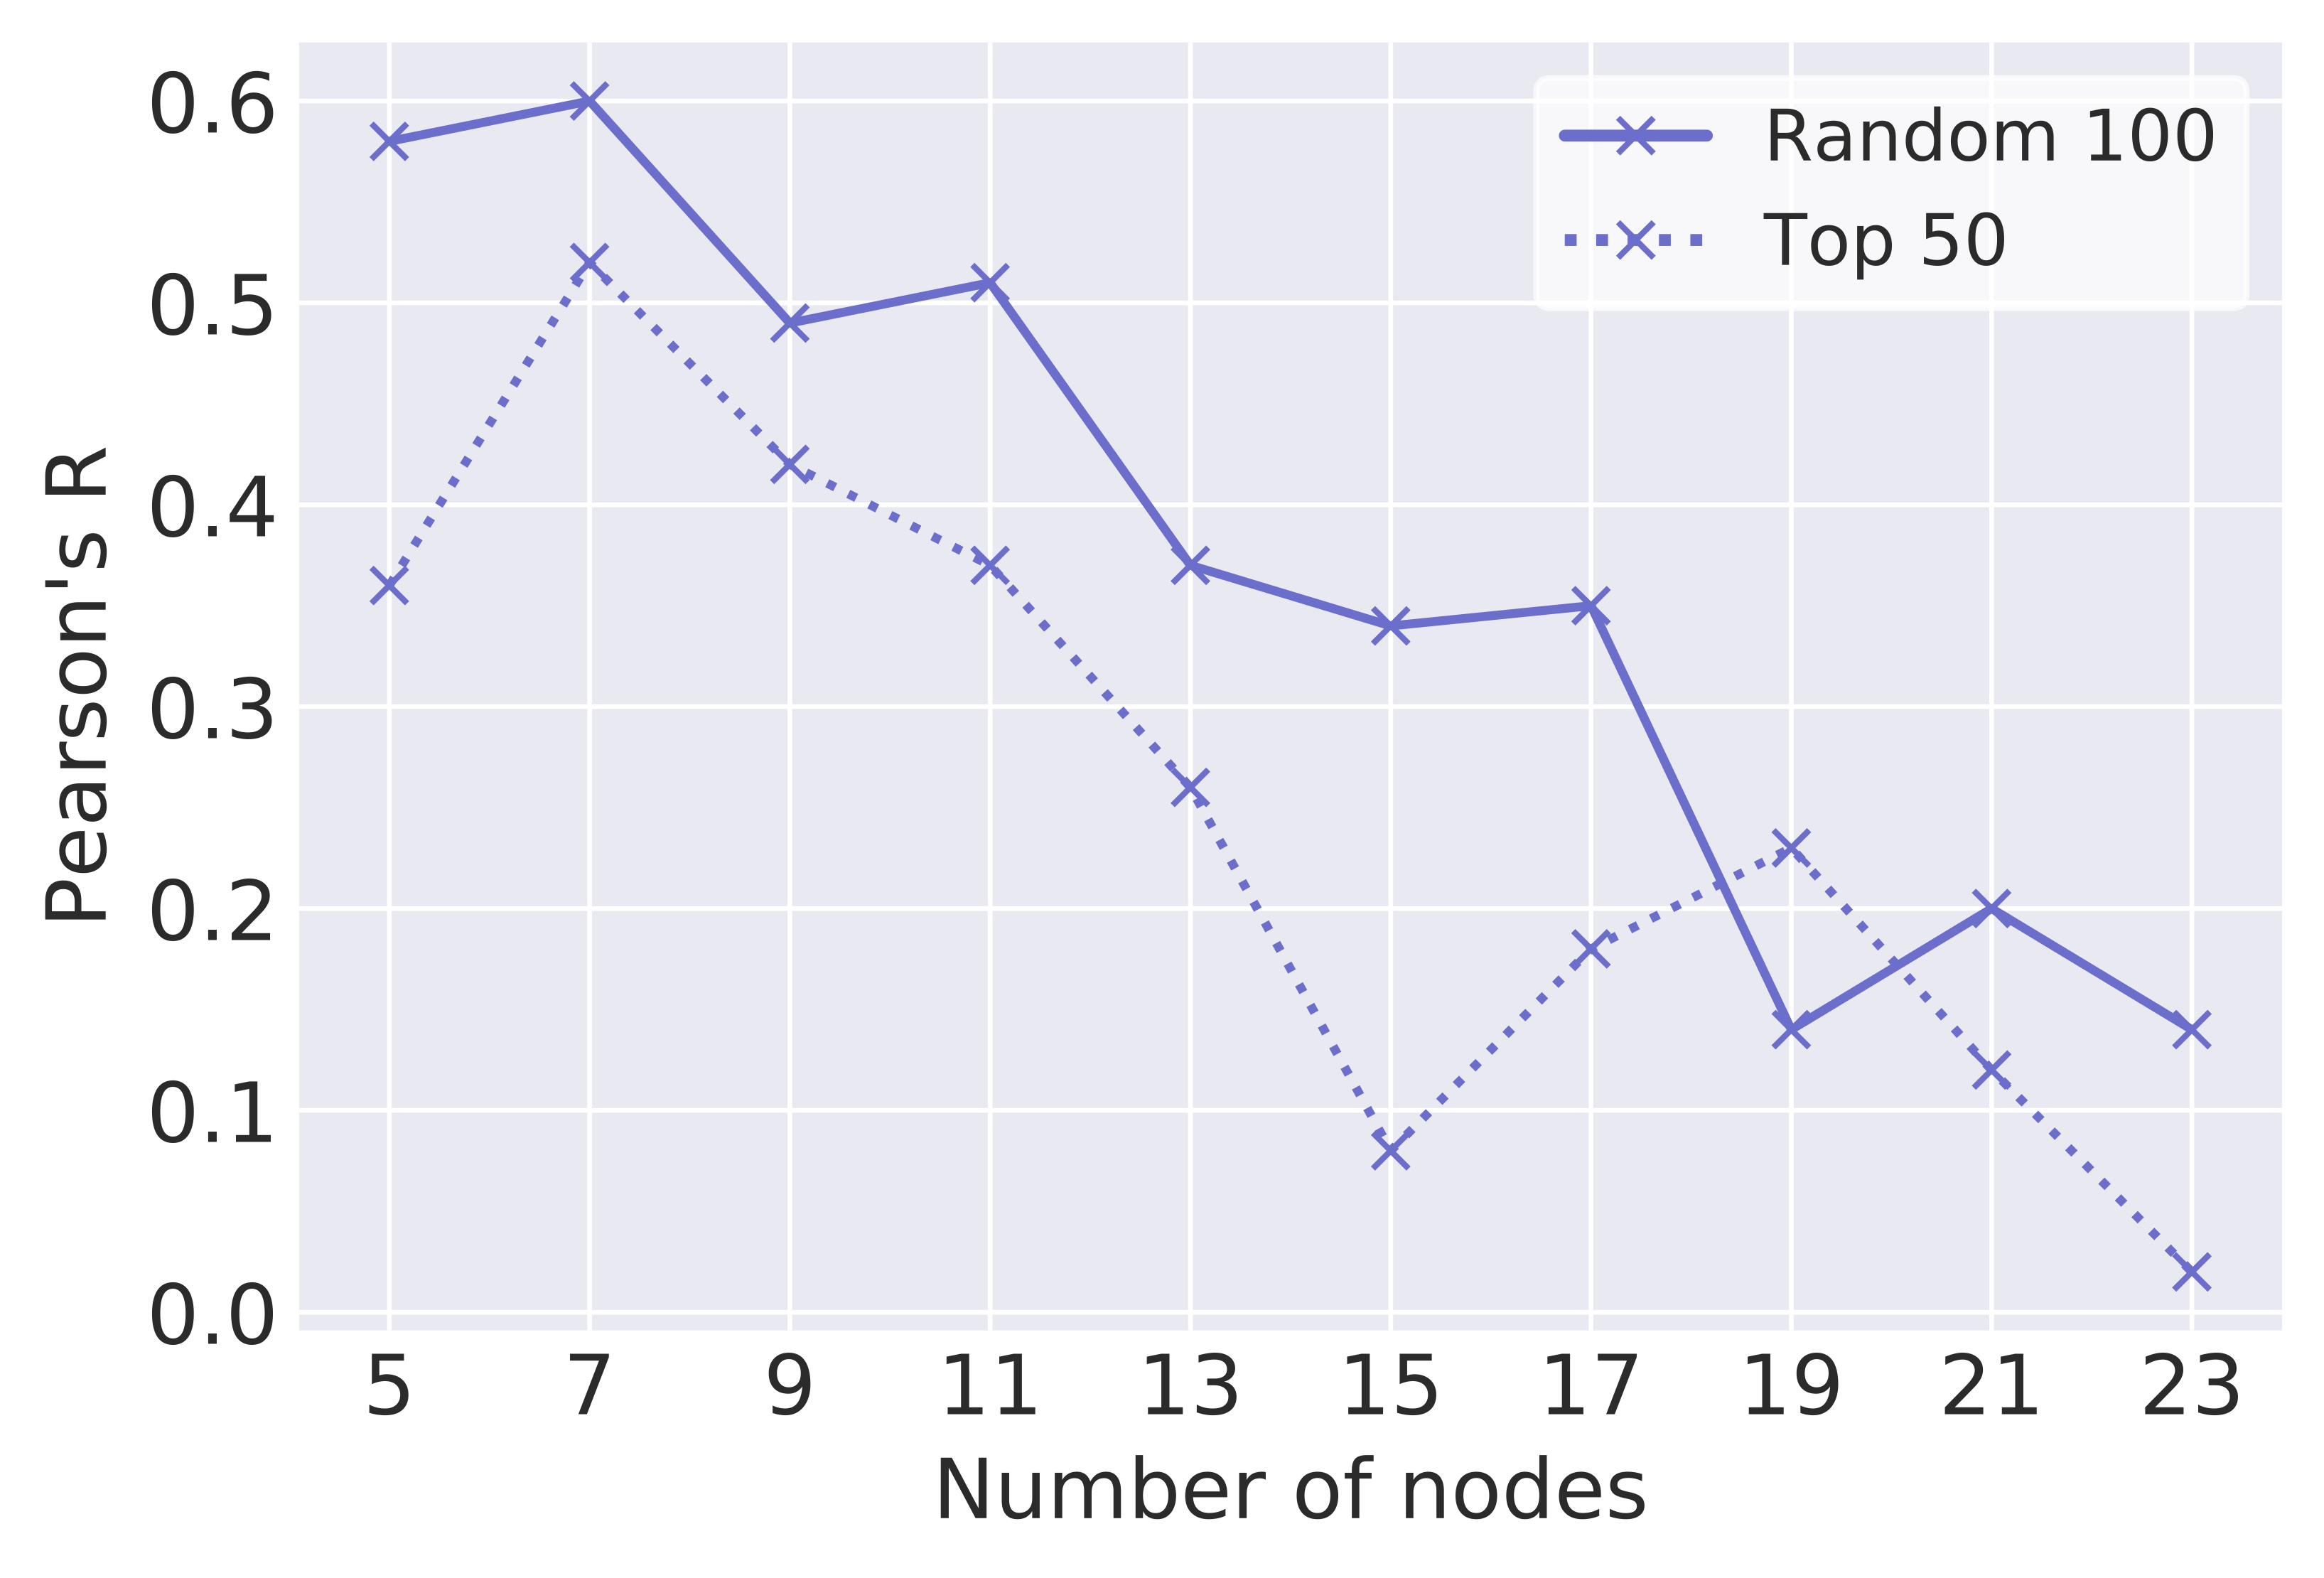
\includegraphics[width=4\linewidth]{figures/nodes.png}
  \caption{Vary number of nodes; $T=5$ , forward-backward}
  \label{fig:sfig2}
\end{figure}
\begin{figure}
  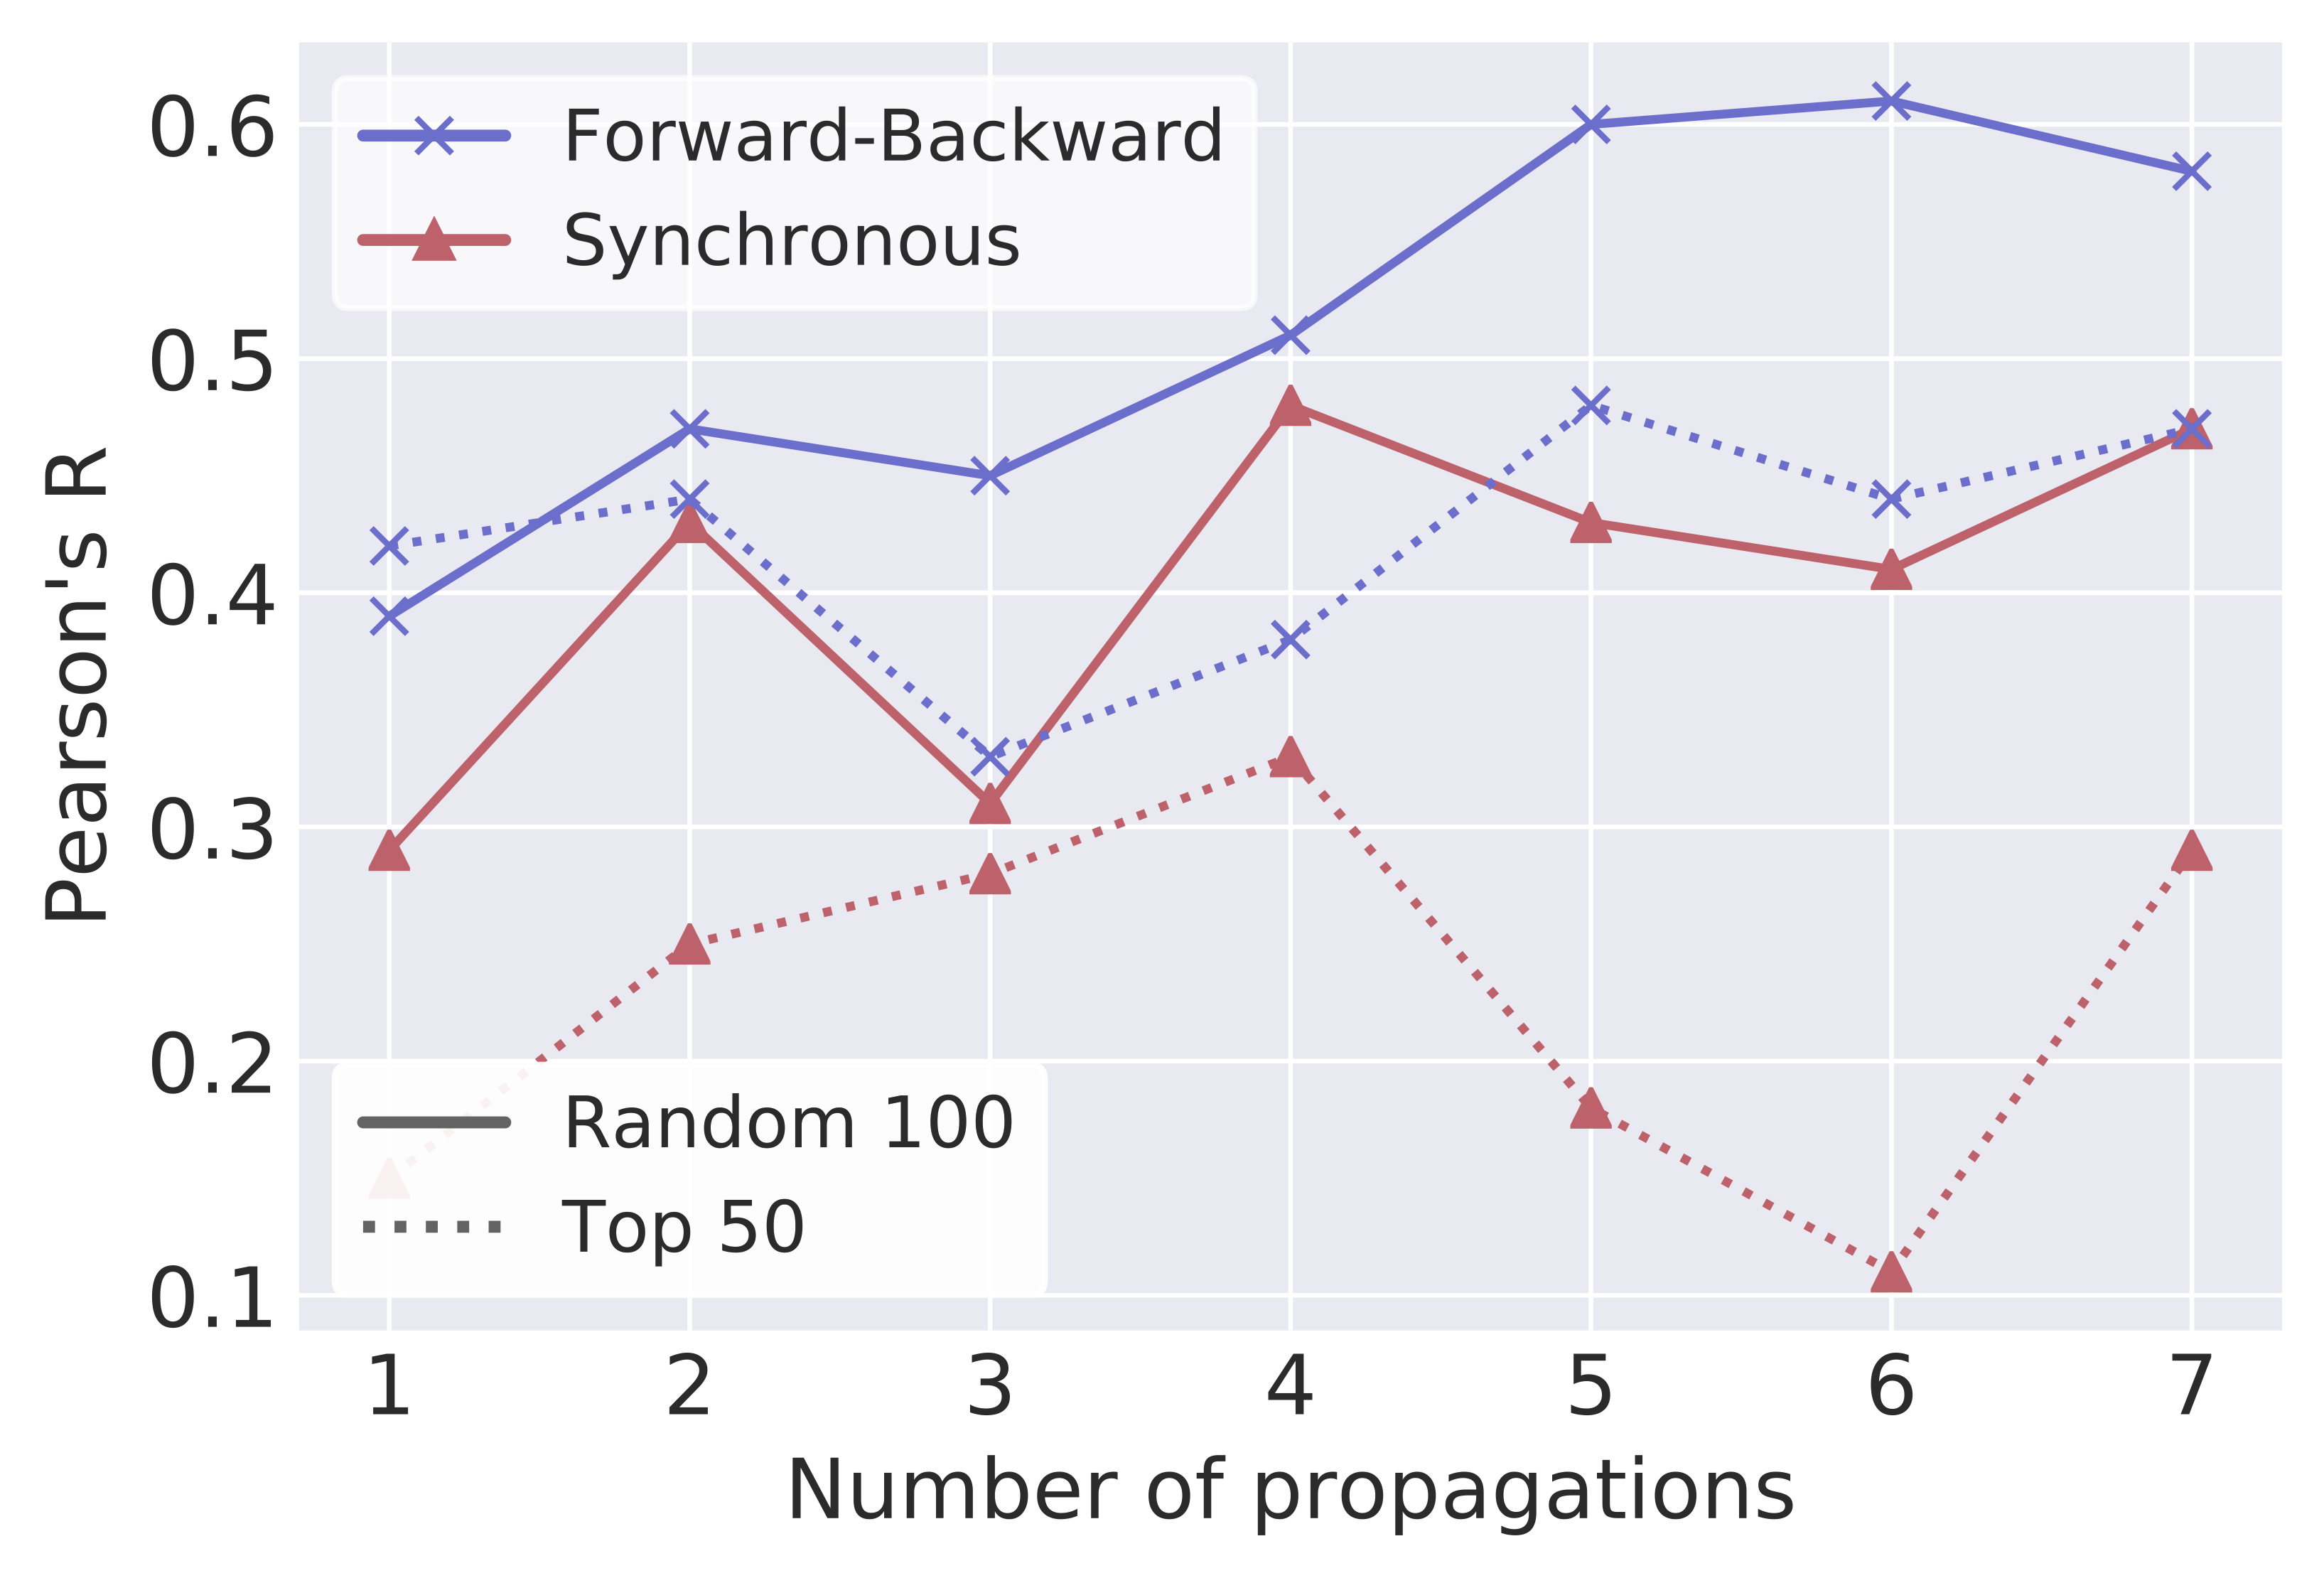
\includegraphics[width=4\linewidth]{figures/tsteps.png}
\caption{ GHN when varying the number of nodes and propagation scheme}
% \label{fig:ghn_hyps}
  \label{fig:sfig1}
\end{figure}
\else
\begin{figure}[t]
\vspace{-1.0cm}
 \begin{center}
\begin{subfigure}{.48\textwidth}
  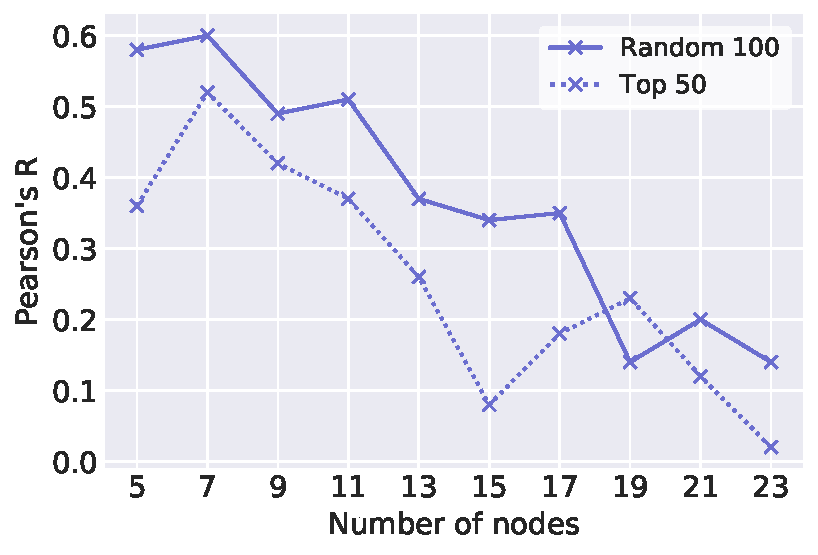
\includegraphics[width=0.8\linewidth]{figures/nodes.pdf}
  \caption{Vary number of nodes; $T=5$ , forward-backward}
  \label{fig:sfig2}
\end{subfigure}
\begin{subfigure}{.48\textwidth}
  \centering
  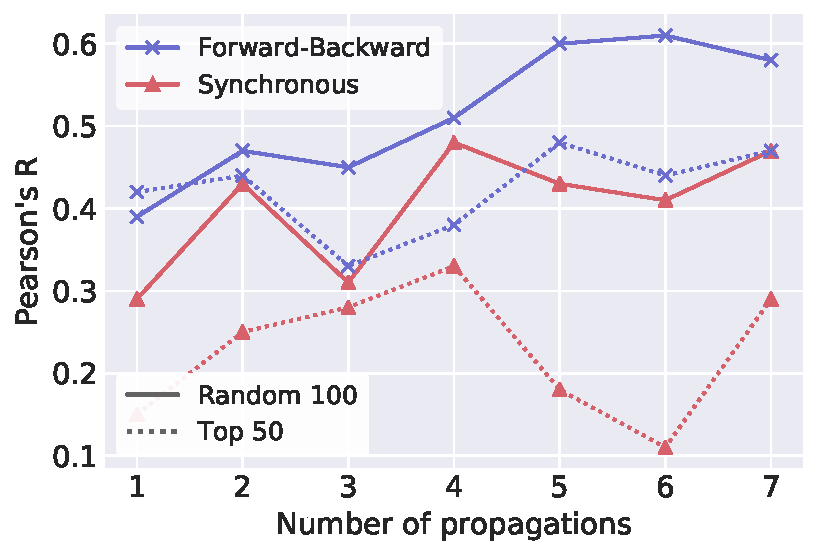
\includegraphics[width=0.8\linewidth]{figures/tsteps.pdf}
  \caption{Vary propagation schemes, $N=7$ }
  \label{fig:sfig1}
\end{subfigure}%
\caption{ GHN when varying the number of nodes and propagation scheme}
\label{fig:ghn_hyps}
\end{center}
\vspace{-0.5cm}
\end{figure}
\fi

\vspace{-0.25cm}
\paragraph{Number of graph nodes:}
The GHN is compatible with varying number of nodes - graphs used in training need not be the same
size as the graphs used for evaluation. Figure~\ref{fig:sfig2} shows how GHN performance varies as a
function of the number of nodes employed during training - fewer nodes generally produces better
performance. While the GHN has difficulty learning on larger graphs, likely due to the vanishing
gradient problem, it can generalize well from just learning on smaller graphs. Note that all GHNs
are  tested with the full graph size ($N=17$ nodes).

\vspace{-0.25cm}
\paragraph{Number of propagation steps:}
We now compare  the forward-backward propagation scheme with the regular synchronous propagation
scheme. Note that $T=1$ synchronous step corresponds to one full forward-backward phase. As shown in
Figure~\ref{fig:sfig1},  the forward-backward scheme consistently outperforms the synchronous
scheme. More propagation steps also help improving the performance, with a diminishing return. While
the forward-backward scheme is less amenable to acceleration from parallelization due to its
sequential nature, it is possible to parallelize the evaluation phase across multiple GHNs when
testing the fitness of candidate architectures.

\begin{wraptable}[8]{r}{5.5cm}
\iflatexml
\else
\footnotesize
\fi
\vspace{-0.4cm}
\begin{center}
\begin{tabular}{ c c c c} 
SP & PE & \multicolumn{2}{c}{Correlation}    \\ 
 &&  Random-100 & Top-50   \\ 
\hline
\xmark & \xmark & 0.24 & 0.15\\
\xmark & \cmark  &  0.44 & 0.37\\
\cmark & \cmark  & 0.68 & 0.48 
\end{tabular}
\end{center}
\vspace{-0.1in}
\caption{Stacked GHN Correlation. SP denotes share parameters and PE denotes passing embeddings}
\label{table:stacked}
\end{wraptable}

\vspace{-0.25cm}
\paragraph{Stacked GHN for architectural motifs:}
We also evaluate different design choices of GHNs on representing architectural motifs. We compare
1) individual GHNs, each predicting one block independently, 
2) a stacked GHN where individual GHN's
   pass on their graph embedding without sharing parameters, 
3) a stacked GHN with shared parameters (our proposed approach). 
As shown in Table~\ref{table:stacked},  passing messages between GHN's is crucial, and sharing parameters produces better performance.